% 2. RAG Entwicklung, welche Frameworks gibt es 
% -> Konfigurierbarkeit durch Files
% -> Maintainability
% -> Beliebtheit?
% -> Future Work (Haystack UI)
% -> Modularität (nach Gao.)
% -> IRA Methoden


Developing retrieval-augmented generation systems is a difficult task that needs several reconfiguration phases.\cite{Simon.10112024} Component evaluation and in-depth failure analysis are key requirements for readjusting the right parts within the RAG-system, as they can include complex pipelines that may involve iterative or recursive processes. Failures can occur in many parts of the RAG-system. Barnett et al.\cite{Barnett.2024} created a list of 7 failures occuring in an advanced RAG system with Rewrite-Retrieve-Rerank-Read (4R) structure as Gao et al.\cite{Gao.18.12.2023} has defined it. Therefore for a framework it is indespensible to evaluate all components next to the end-to-end evaluation for the overall result. In this chapter, we will discuss how fast RAG development with transparent and reproducible results can be done. At first we will introduce Haystacks approach of fast RAG development. Secondly we will present classification metrics for end-to-end evaluation. Then we introduce failure types in RAG-systems and how to evaluate them. Lastly we will introduce the novelle blueprint by Simon et al.\cite{Simon.10112024} for handling external validity in RAG experiments. 

\section{Fast RAG Development}

\begin{figure}[b]
    \centering
    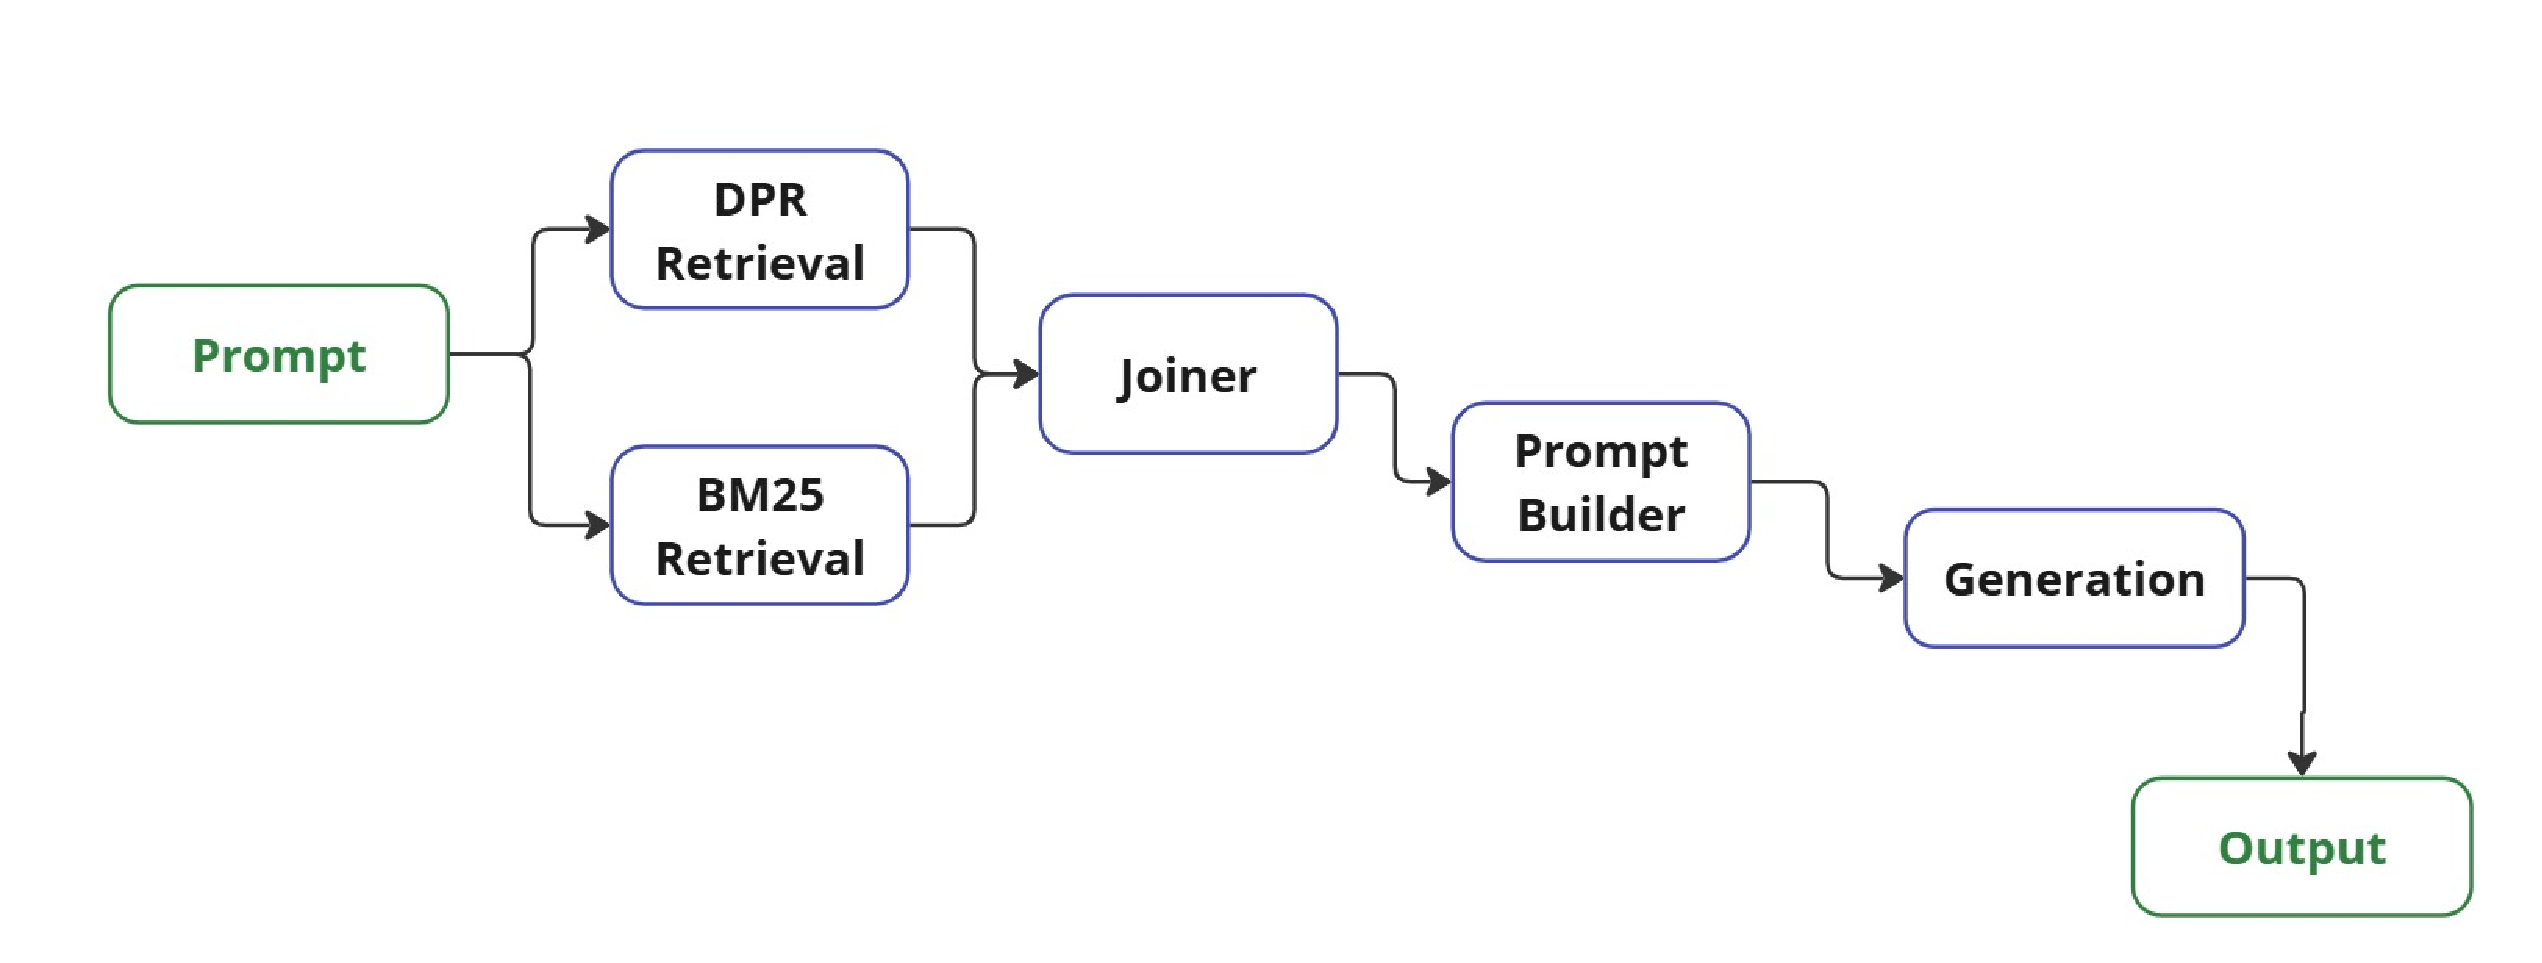
\includegraphics[width=\textwidth]{images/showcase-pipeline.pdf}
    \caption{A simple Retrieve-Read pipeline with both dense and sparse retrieval.}
    \label{fig:showcase}
\end{figure}


There are several RAG development tools and frameworks. Highly used ones are Llama-Index\cite{Liu_LlamaIndex_2022}, Langchain\cite{Chase_LangChain_2022} and Haystack\cite{Pietsch_Haystack_the_end-to-end_2019}. All of them offer comparable functionality for building advanced RAG systems in modularized architecture as introduced by Gao et al.\cite{Gao.18.12.2023}. Haystack does offer a functionality, where users can define a pipeline via a YAML-file. This enhances the reconfiguration of such systems, because instead of editing python files, there are just parameters in a YAML to be changed. This enhances the ability to report the methodologies of each experiment too. Instead of saving a python script or module for each configuration, only a YAML is stored that describes the tested RAG architecture fully. An example of this YAML definition can be seen in figure \ref{fig:showcase} and the YAML code below.

Furthermore Haystack comes with router components (cf. router component, section \ref{sec:router}) and the ability to create custom components, which enables iterative, recursive and adaptive RAG functionalities. Components in the Haystack universe can be seen as nodes of an RAG pipeline such as a generator or a retriever. 

\newpage
\begin{minted}[
    frame=single,
    bgcolor=lightgray
  ]{yaml}
components:
  llm:
    init_parameters:
      api_base_url: null
      api_key:
        env_vars: OPENAI_API_KEY
      ...
  prompt_builder: ...
  bm25_retriever: ...
  embedding_retriever: ...
  joiner: ...
  text_embedder: ...
  docs_embedder: ...
connections:
- receiver: llm.prompt
  sender: prompt_builder.prompt
- ...
\end{minted}

\textcolor{red}{Wie werde ich das nutzen?}

\section{Evaluating RAGs}

\textcolor{blue}{Here comes Citavi section Why E2E and Comp Evaluation? Erstelle Beispiel, welches zeigt das E2E nicht zeigt, WARUM ein generierter Response nicht die korrekt Antwort hat (zB fehlendes Dokument im Retrieval)}

\paragraph{End-to-End Evaluation}

Accelerating this time-consuming process is needs evaluation of all components and fast RAG configuration.\cite{Ru.15.08.2024.} Eventhough all components of a RAG-system affect its overall performance, there are ones that can not be evaluated directly.  \\
\begin{itemize}
    \item LLM + RAG Baselines
    \item End-to-End Metrics
    \item Evaluation Approach
\end{itemize}


\paragraph{Component Evaluation}

\begin{itemize}
    \item 7 Failures
    \item How to Evaluate those
\end{itemize}

\section{Increasing Transparency in RAG Experiments}

\begin{itemize}
    \item DVC for RAG Experiments
    \item Save YAMLs, Versionize Data + Code
\end{itemize}

\section{External Validity of RAG Experiments}

\begin{figure}
    \centering
    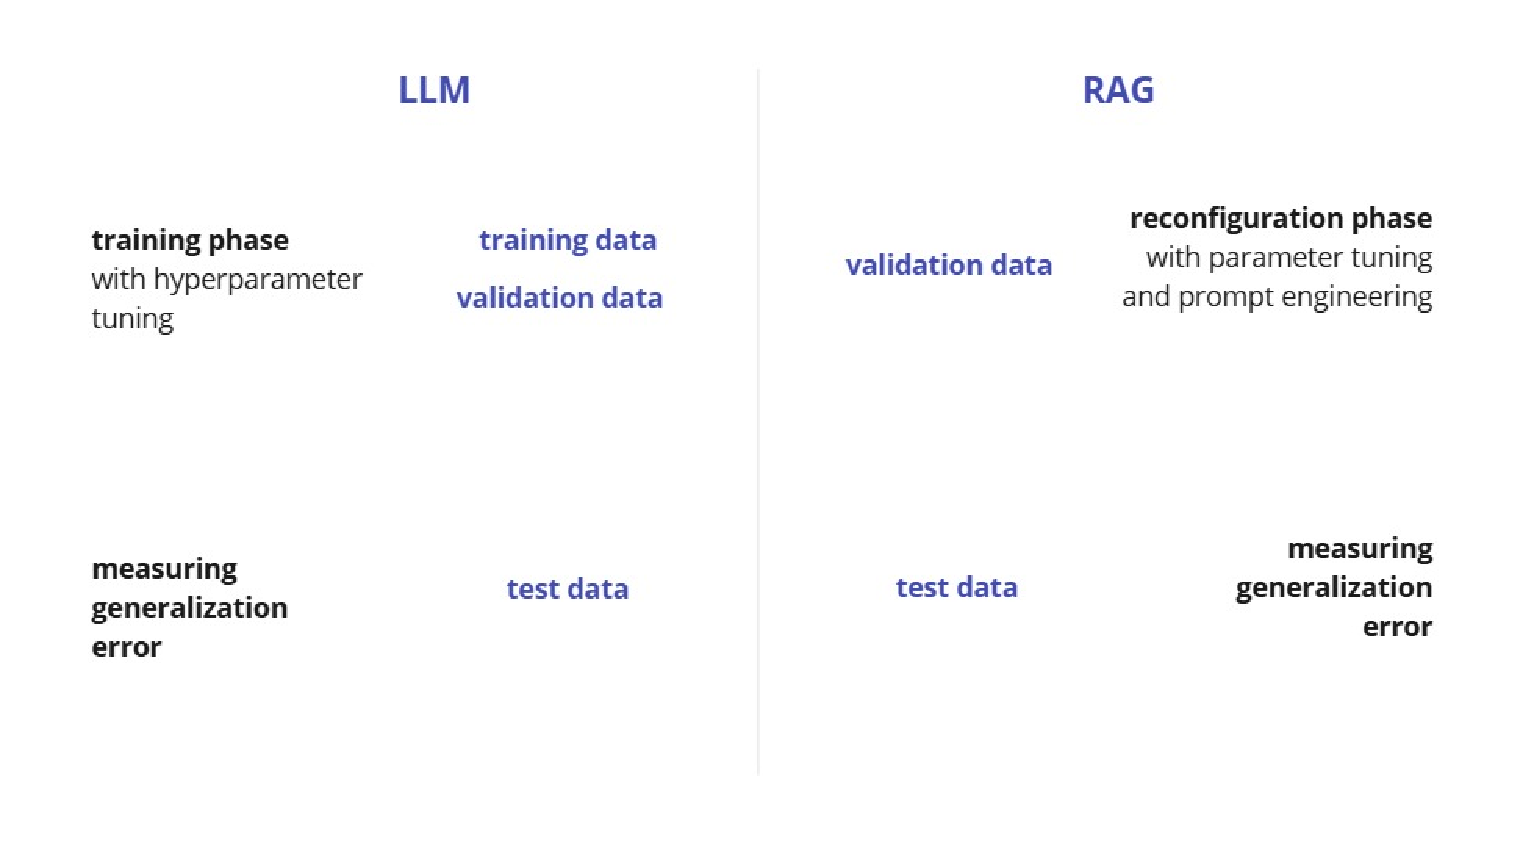
\includegraphics[width=\textwidth]{images/RAGvsLLM-tuning.pdf}
    \caption{Comparison of reconfiguration between RAGs and LLMs - both relying on tuning parameters and test data.}
    \label{fig:tuning}
\end{figure}


Data is rare, especially for down-stream tasks in domains such as configuration validation or similar tasks. They often rely on few datasets that can not represent the whole domain. Therefore there are measures required to ensure that the developed systems can be generalized from the seen data to the unseen production data. Measuring generalization error in the large language model development is done by splitting the data into training, validation and test datasets. While the training and validation data is used for hyperparameter tuning to ensure the best performing model, the test dataset on the other hand is used to check if the hyperparameter tuning introduced an overfitting. This procedure must be adopted for RAG systems too (cf. figure \ref{fig:tuning}). Even though they do not rely on a training in the most cases, the continous reconfiguration of such systems, including prompt engineering or parameter tuning can lead to differences in seen and unseen data. The needs for a test dataset is independent from a potential training phase, but instead very dependent on a tuning phase for the systems, that is done till the results converge to the best outcoming scenario. Both LLM and RAG development share those reconfiguration phases. 


\paragraph{RAG Evaluation needs a Holdout-Testset}
\begin{itemize}
    \item RAG Experiments belongs to ML Experiments 
    \item Requires Seeding
    \item ML Experiments might cause Overfitting
    \item Generalization (External Validity) is testable with a hard data split (train vs validation vs test)
    \item training data split is not needed, but validation and test is required
    \item validation is for hyperparameter tuning important, which configs have the best results
    \item no testset -> no generalization estimatation
    \item \textcolor{red}{Problem zum Nachdenken} Im Training braucht es ein Holdout-Testset damit man das LLM auswählen kann, welches den geringsten Testfehler hat, aber im RAG wird nicht trainiert. Müssen dann alle Konfigurationen dagegen getestet werden?
\end{itemize}


\section{CLI}

\begin{figure}[!ht]
    \centering
    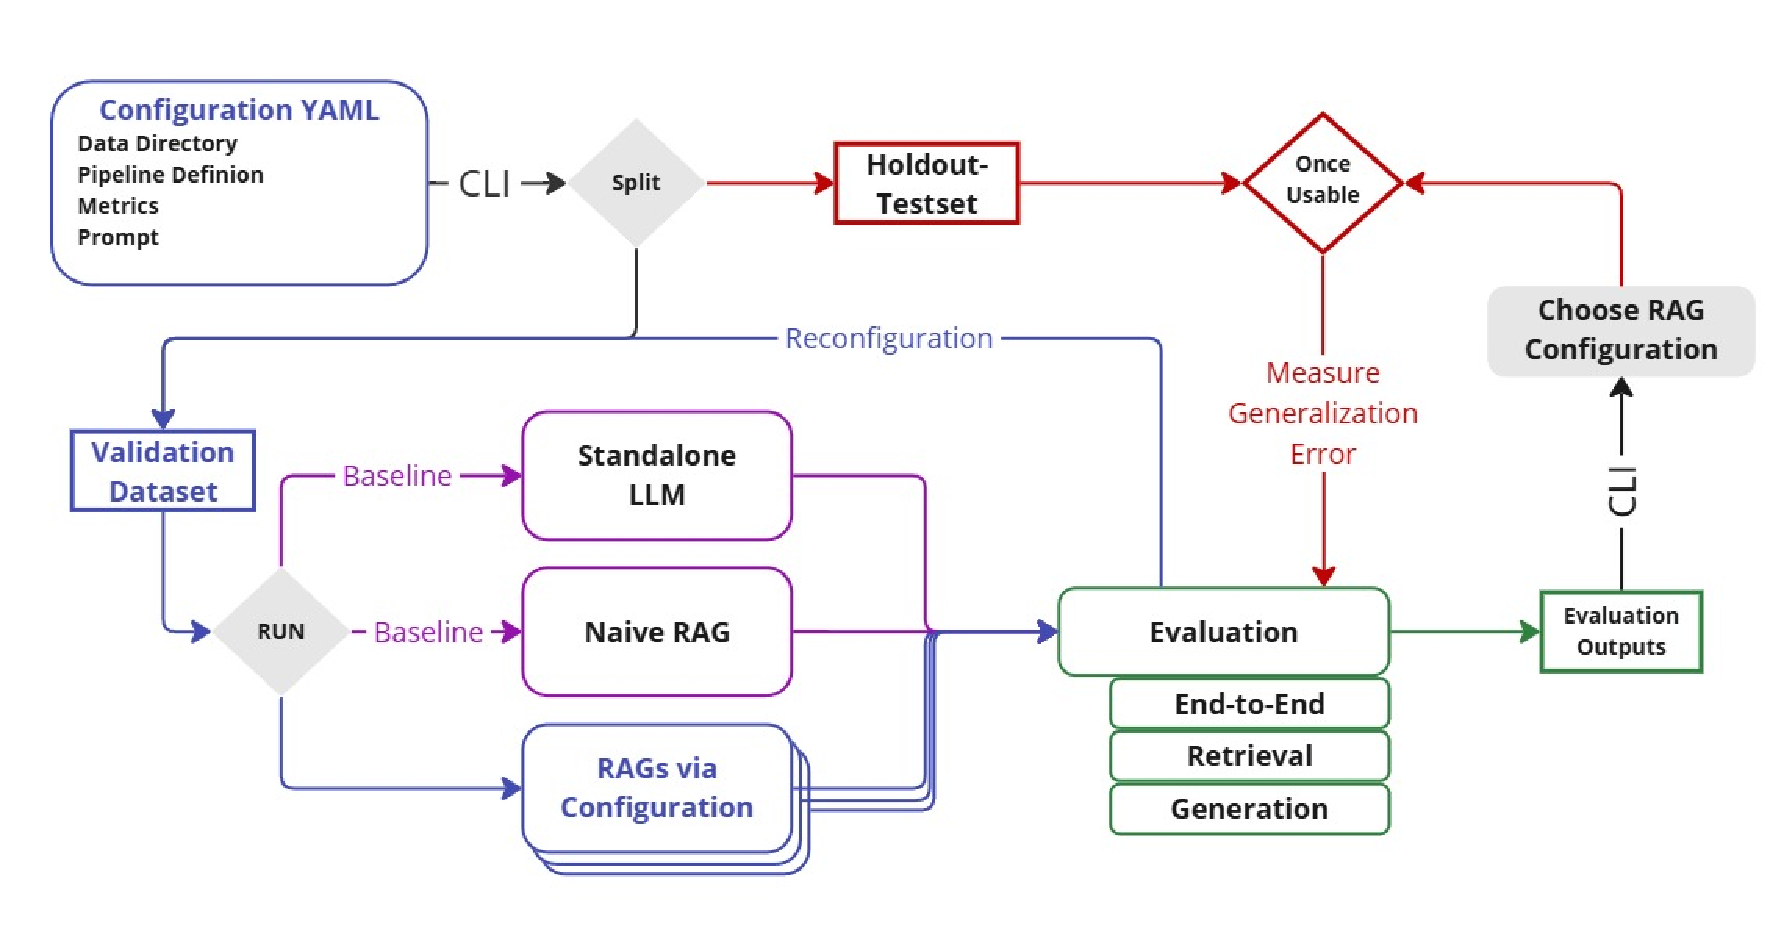
\includegraphics[width=\textwidth]{images/Sketch.pdf}
    \caption{...}
    \label{fig:EvaluationDesign}
\end{figure}

We use the presented Haystack functionalities to build a CLI-based framework around it. Our complete appraoch can be seen in figure \ref{fig:EvaluationDesign}. Given a data directory, pipeline and metrics definition, we first split the data into a validation and holdout-test dataset based on a split parameter \textit{test\_size}. Next we use the resulting validation dataset to run the first evaluations on the data. For that it loads the pipeline and data from its paths and starts with evaluating against a standalone LLM to have a baseline if RAG at all is a significant improvement in contrast to having just an LLM. Next, it ingests data into a vector database and builds an naive RAG with (Retrieve-Read) architecture as another baseline in contast to the in the YAML file defined advanced RAG architecture. The same procedure starts with the RAG configuration from the file. Each run gets evaluated in respect to End-to-End evaluation and component-wise. Evaluations are visualized in \textcolor{red}{EVAL INFOS EINFÜGEN Framework oder PRozess für Indepth Failure Analysis hier erklären}. After failure analysis, the RAG can be reconfigured again to test new parameters. 

\textcolor{blue}{Here comes text how to use Holdout-Test dataset}



\section{Limitations}

List of possible Limitations

\begin{itemize}
    \item Generation Tasks 
    \item Chunking Reconfiguration
\end{itemize}